\documentclass[aspectratio=169]{beamer}
\usepackage{braket,caption}
%\usetheme{focus}
\newcommand{\focus}[1]{\textcolor{blue}{\textbf{#1}}}
\newcommand{\cen}[1]{\begin{center}{#1}\end{center}}

\definecolor{main}{RGB}{40, 40, 40}

\title{
\vspace*{\fill}
\LARGE{Journey from the Hubbard Dimer\\
to the Hubbard Model}
\vspace*{\fill}
}
\vspace*{\fill}
\author{Abhirup Mukherjee, Dr. Siddhartha Lal}
\vspace*{\fill}
\institute{Department of Physical Sciences\\IISER Kolkata}
\vspace*{\fill}
\date{\today}
\vspace*{\fill}
\begin{document}
\begin{frame}{}
\maketitle
\end{frame}

\begin{frame}{Overview of the Process}
\begin{itemize}[<alert@+>]
	\item Choose correlated Anderson model as the auxiliary model and perform URG analysis and extract zero mode to obtain Hubbard dimer as the effective low energy Hamiltonian.
	\item Translate this Hubbard dimer Hamiltonian to recreate a new/renormalized Hubbard model. This Hubbard model is assumed to be linked to the parent Hubbard model via a similarity transformation.
	\item Express equation between renormalized Hubbard and Hubbard dimers as relation between inverse Greens function matrix elements of full Hubbard model and those of the Hubbard dimer.
	\item Obtain Greens functions of the parent Hubbard model in terms of those of the Hubbard dimer.
\end{itemize}
\end{frame}

\begin{frame}{Auxiliary System Approach}
	%\begin{figure}[htpb]
		\centering
		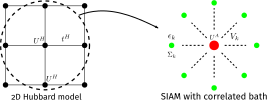
\includegraphics[width=0.7\textwidth]{./cluster-bath.png}
	%\end{figure}
%{\small (SIAM with correlated bath)}

\[\mathrm{Hubbard}~~H^H = -t^H\sum_{\sigma,\left<i,j \right>}\left(c^\dagger_{i\sigma} c_{j\sigma} + \text{h.c.}\right) + U^H\sum_i \tau_{i \uparrow} \tau_{i \downarrow}\]
\[
\mathrm{SIAM}~~H^A = \sum_{k\sigma}\tilde\epsilon_k\tau_{k\sigma} + U^A \tau_{d \uparrow} \tau_{d \downarrow} + U_b \sum_{kk^\prime}\hat n_k \hat n_{k^\prime} -t^A\sum_{k\sigma}\left(c^\dagger_{d\sigma}c_{k\sigma} + \text{h.c.}\right)\]
\[(\tilde{\epsilon}_{k} = \epsilon_{k} + \Sigma (k,\omega)) \]
\end{frame}
\begin{frame}{RG Analysis of Auxiliary System}
	\[H^{A} = \sum_{k\sigma}\tilde\epsilon_k\tau_{k\sigma} + U^{A} \tau_{d \uparrow} \tau_{d \downarrow} + U_b \sum_{kk^\prime}\hat n_k \hat n_{k^\prime} -t^{A}\sum_{k\sigma}\left(c^\dagger_{d\sigma}c_{k\sigma} + \text{h.c.}\right)\]
	\[\Bigg\downarrow U_{A} H^{A} U^{\dagger}_{A}~~(URG)\]
	\[ H ^{A*} = \sum_{k\sigma}^*\left[\tilde\epsilon_k\tau_{k\sigma} -{t}^{A*}\left(c^\dagger_{d\sigma}c_{k\sigma} + \text{h.c.}\right)\right] + U^{A*} \tau_{d \uparrow} \tau_{d \downarrow} + U_{b}^* \sum_{kk^\prime}^*\hat n_k \hat n_{k^\prime} \]
	\[ (U_{b}^{*} = U^{A*}) \]
	\[\Bigg\downarrow \text{zero mode}\]
	\[ H^{D} = -{t}^{D}\sum_{\sigma}\left(c^\dagger_{d\sigma}c_{z\sigma} + \text{h.c.}\right) + U^{D} (\tau_{d \uparrow} \tau_{d \downarrow} + \tau_{z \uparrow} \tau_{z \downarrow}) \]
\end{frame}
\begin{frame}{Restoring Translational Invariance}
\begin{minipage}{0.55\textwidth}
	\centering
	\[\tilde H(\tilde t, \tilde U) = \frac{2}{Nw}\sum_{\left<ij \right>}H^D(i,j)\]
	\[H^D = -{t}^D\sum_{\sigma}\left(c^\dagger_{i\sigma}c_{j\sigma} + \text{h.c.}\right) + U^D\left(\tau_{i \uparrow} \tau_{i \downarrow} + \tau_{j \uparrow} \tau_{j \downarrow}\right)\]
	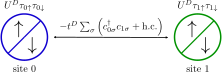
\includegraphics[width=0.75\textwidth]{./hubb_dim.png}
	\[\tilde t \equiv \frac{2}{Nw}t^D, \quad\tilde U \equiv \frac{2}{Nw}U^D\]
\end{minipage}
\hspace*{\fill}
\begin{minipage}{0.4\textwidth}
	\centering
	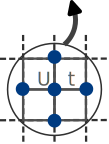
\includegraphics[width=0.9\textwidth]{./tiling.png}\\
	\vspace*{-20pt}
	{\small (Tiling 2D square lattice with dimers)}\\
	{\small ($N$ sites, $w$ coordination number)}
\end{minipage}
\end{frame}
\begin{frame}{Relating the original and reconstructed Hubbard models}
\begin{itemize}
\item We chose an auxiliary model appropriate to the original Hubbard model ($H^{H}$).
\item We then performed the URG on it, and took the zero mode of the stable fixed point theory to obtain a Hubbard dimer. 
\item Finally, we tiled the 2D square lattice with the dimer to obtain a reconstructed Hubbard model ($\tilde{H}$) with new parameters. 
\end{itemize}
In principle, $H^{H}$ and $\tilde{H}$ are related via a unitary (or atleast similarity) transformation.
\[\tilde H = \mathcal{U}H^H\mathcal{U}^{-1}~~,~~ \mathcal{U} = T Z U_{A}\]
\[Z:~\mathrm{zero~mode~projection}~,~ T:~\mathrm{lattice~tiling~operation}\] 
\[\therefore~\tilde G (\tilde r,\tilde r^\prime) = G^H ( r, r^\prime)\]
\[\left(\text{where }\ket{\tilde r} \equiv \mathcal{U}\ket{r}\right)\]
\end{frame}

\begin{frame}{Inverse Greens function from Hamiltonian}
	\only<1>{
	\cen{\focus{Write equation in terms of inverse Greens function \(G^{-1}(\omega) = \omega - H\)}}
	\begin{equation*}\begin{aligned}
		\omega - \tilde G^{-1} &= \frac{2}{Nw}\sum_{\left<ij \right>}\left[\omega - G^{-1}_D(\omega, i, j)\right]\\
	\longrightarrow \tilde G^{-1} &= \frac{2}{Nw}\sum_{\left<ij \right>}G^{-1}_D(\omega, i, j)
\end{aligned}\end{equation*}
}
	\only<2-4>{\[\tilde G^{-1} = \frac{2}{Nw}\sum_{\left<ij \right>}G^{-1}_D(\omega, i, j)\]
\begin{itemize}
	\only<2>{\item Take diagonal matrix element \(\bra{\tilde i}G^{-1}\ket{\tilde i}\), against excitations above the \textit{exact ground state}:
		\[\ket{\tilde i} \equiv \mathcal{U}\ket{i} = \mathcal{U}c^\dagger_i \ket{0}\]
On the RHS, there are \(w\) terms that have the index \(i\).
	\begin{equation*}
		\left(\tilde G^{-1}\right)_{\tilde i, \tilde i} = \left(G^{-1}\right)_{i,i} = \frac{2}{Nw}\times \left(G_D^{-1}\right)_{ii}\times w = \frac{2}{N}\left(G_D^{-1}\right)_{00} \equiv g_0
	\end{equation*}
	\begin{center}
	(due to translation invariance)
	\end{center}
}
\only<3>{\item Take nearest-neighbour matrix element \(\bra{\tilde i}\tilde G^{-1}\ket{\tilde j}\). On the RHS, there's just one term that has both indices \(i\) and \(j\).
	\begin{equation*}
		\left(\tilde G^{-1}\right)_{\tilde i, \tilde j} = \left(G^{-1}\right)_{i, j} = \frac{2}{Nw}\times \left(G_D^{-1}\right)_{ij} = \frac{2}{Nw}\left(G_D^{-1}\right)_{01} \equiv g_1
	\end{equation*}
	\begin{center}
	(due to translation invariance)
	\end{center}
}
\only<4>{\item \focus{All other matrix elements are zero}, because no term in the Hamiltonian scatters between non-nearest-neighbour sites \\
	\(\longrightarrow\) \focus{inverse Greens function matrix has contributions only from nearest neighbour sites, and respects the lattice geometry}
}
\end{itemize}
}
\end{frame}

\begin{frame}{Diagonalizing the inverse Greens function matrix}
	\only<+>{
	\begin{equation*}
		G^{-1} = \begin{pmatrix} g_0 & g_1 & 0 & ... & g_1 \\
			g_1 & g_0 & g_1 & 0 & ... \\
			 0   & g_1 & g_0 & g_1 & ...\\
			  0  & 0 & ... &&
	\end{pmatrix} 
	\xrightarrow{\text{Fourier transform to $k-$space}}
			g_0 + g_1\begin{pmatrix} \xi_{\vec k_1} & 0 & 0 &...\\
				0& \xi_{\vec k_2} & 0 &...\\ 
				0 & 0 & \xi_{\vec k_3} &...\\
				0 &0 & ...&
	\end{pmatrix}
\end{equation*}
\[\xi_{\vec k} = \sum_\text{i=1}^w \cos (a_i k_i)\]
\[k_i \equiv \text{ projection of $\vec k$ on the $i^\text{th}$ primitive vector}, a_i \equiv \text{ lattice spacing along $i^\text{th}$ dimension}\]
\cen{$\xi_{\vec k}$ arises from lattice geometry and \focus{introduces non-locality in $G^{-1}$}.}
}
\only<2>{
{\large
\begin{equation*}
	G^{-1} = g_0 + g_1\begin{pmatrix} \xi_{\vec k_1} &&&\\
				& \xi_{\vec k_2} &&\\ 
				&& \xi_{\vec k_3} &\\
				&&&
	\end{pmatrix}
		\xrightarrow{\text{invert the diagonal matrix}}
		G = \begin{pmatrix} G_{\vec k_1} &&&\\
				& G_{\vec k_2} &&\\ 
				&& G_{\vec k_3} &\\
				&&&  \end{pmatrix} 
\end{equation*}
}
}
\end{frame}
\begin{frame}{Single-particle Greens functions and related quantities}
\large
\begin{equation*}\begin{aligned}
	\only<1-4>{
	\text{\focus{$\color{blue}{\vec k}$-space Greens function: }} G_H (\vec k, \omega) &= \frac{N}{2}\left\{\left[G_{D}^{-1}(\omega)\right]_{00} + \frac{1}{w}\left[G_{D}^{-1}(\omega)\right]_{01}\xi_{\vec k}\right\}^{-1}\\[20pt]}
	\only<2-4>{
	\text{$\color{blue}{\vec r}$\focus{-space Greens function: }} G_H (\vec r, \omega) &= \sum_{\vec k}\frac{e^{i \vec{k}\cdot\vec{r}}}{2}\left\{\left[G_{D}^{-1}(\omega)\right]_{00} + \left[G_{D}^{-1}(\omega)\right]_{01}\frac{\xi_{\vec k}}{w}\right\}^{-1}\\[20pt]}
	\only<3-4>{
	\text{\focus{self-energy: }} \Sigma_H (\vec k, \omega) &= \omega - g_0 + \left(t^H - g_1\right)\xi_{\vec k}\\[20pt]}
\only<4-4>{
	\text{\focus{Spectral function: }} A_{H}(\vec{k},\omega) &= -\frac{1}{\pi} \textrm{Im}(G_{H}(\vec{k},\omega)) = -\frac{1}{\pi} \textrm{Im}\left[ (g_{0} + g_{1}\xi_{\vec{k}})^{-1}\right]
}
\end{aligned}\end{equation*}
\end{frame}

\begin{frame}{On the Bethe Lattice $(w \to \infty)$}
\begin{minipage}{0.59\textwidth}
\centering
\only<+>{
Hamiltonian scaling arguments suggest \footnotemark
\begin{equation*}
%	G_{ij} = G_{ii}\delta_{ij}
t^{H} \to t^{H}/\sqrt{w}
\end{equation*}
\begin{itemize}
	\item In an auxiliary model treatment of the Hubbard model on this lattice, \focus{there is only one (direct) path linking the impurity to a given neighbouring bath site.}\\[10pt]
\item This ensures that the impurity self-energy is related \focus{simply to the local part of the bath Greens function.}
\end{itemize} 
}
\only<+>{
A locality also emerges from our formulation:

\begin{equation*}
G^{-1}_{ii} = \frac{2}{N}\left[G^{-1}_D\right]_{00} \to \text{finite}
\end{equation*}
\begin{equation*}
	\mathbf{\textcolor{blue}{G^{-1}_{ij} = \frac{2}{Nw}\left[G^{-1}_D\right]_{00} \to 0}} \quad\text{ when } w \to \infty
\end{equation*}
\\[20pt]


\(G^{-1}_{ij}\) becomes diagonal
\(\longrightarrow \color{blue}{G_{ij}} \) \focus{becomes diagonal}
\[\Sigma_H (\vec k, \omega) \to \omega - g_0 + t^H \xi_{\vec k} \]
}
\end{minipage}
\begin{minipage}{0.4\textwidth}
	\centering
	\includegraphics[width=0.7\textwidth]{./bethe.png}\\[20pt]
	Bethe lattice with \(w=3\)\\[10pt]
	No non-trivial loops on this lattice. Any pair of sites $(i,j)$ are only connected via a direct path (if it exists).
\end{minipage}
\footnotetext{Vollhardt, Krzysztof and Marcus, Dynamical Mean-Field Theory, 2012, Springer Berlin Heidelberg}
\end{frame}
\begin{frame}{Choosing ground state wavefunctions}
Note that our formulation is in principle exact if we use the exact ground state eigenfunction of the Hubbard model. Putting this into practice is however difficult.
\end{frame}
\begin{frame}{Choosing ground state wavefunctions}
\begin{itemize}
\item These are some strategies for choosing the ground state with which to measure the Greens functions:
\end{itemize}
%\vspace*{\fill}
\begin{itemize}
	\only<+>{
	\item Localized limit: \[\ket{\tilde 0} = \sum_{\left<ij \right>}\ket{0^D_{ij}}\otimes\ket{\Phi}\]
		\begin{itemize}
			\item Analytic expressions for $g_0$ and $g_1$
			\item However, reduction of many-particle entanglement to only short-ranged
		\end{itemize}
	}
	\only<+>{
	\item Compute exact wavefunctions numerically for given values of $U^H$ and $t^H$:
		\begin{itemize}
			\item In principle exact, however size of lattice has to be small to allow exact diagonalization (or any other numerical method)
			\item High accuracy but no analytical insight
		\end{itemize}
	}
	\only<+>{
	\item Improve the wavefunction by connecting the Hubbard dimer to a bath:
		\begin{minipage}{0.65\textwidth}
		\[\underbrace{H^D}_\text{Hubbard dimer} + \underbrace{\sum_{k\sigma}\epsilon_{k\sigma}\tau_{k\sigma}}_\text{bath} \quad \underbrace{- t \sum_{k\sigma}\left(c^\dagger_{\tilde i\sigma}c_{k\sigma} + c^\dagger_{\tilde j\sigma}c_{k\sigma} + \text{h.c.}\right)}_\text{bath-dimer hybridisation}\]
		\begin{itemize}
			\item Allows systematic improvement by increasing number of momentum states in bath
			\item Introduces more entanglement, because the electrons of the dimer can now traverse through the bath
			\item Introduces a three peak spectral function , and hence of observing a metal-insulator transition
		\end{itemize}
		\end{minipage}
		\hspace*{\fill}
		\begin{minipage}{0.25\textwidth}
			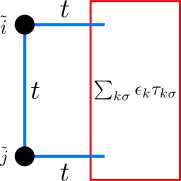
\includegraphics[width=0.9\textwidth]{./dimer_dispersion.png}
		\end{minipage}
	}
	\only<+>{
	\item Further improve the wavefunction by introducint self-energy into the bath:
		\begin{minipage}{0.65\textwidth}
			\[\epsilon_k \to \epsilon_k + \Sigma(k, \omega)\]
		\begin{itemize}
			\item Singular $\Sigma$ would introduce gap in bath spectrum and potentially lead to insulating phase
			\item Regular $\Sigma$ (for eg., $\sim \omega^2$) allows low energy excitations and might result in metallic phase
			\item Overall, greater control over the physics
		\end{itemize}
		\end{minipage}
		\hspace*{\fill}
		\begin{minipage}{0.25\textwidth}
			\includegraphics[width=0.9\textwidth]{./dimer_dispersion_selfenergy.png}
		\end{minipage}
	}
\end{itemize}
\end{frame}

\begin{frame}{Future Goals}
	\begin{itemize}
		\item Obtain expressions for two-particle Greens functions, in order to study holon/doublon excitations
		\item Recreate the metal-insulator transition for the Hubbard model on (say) the 2D square lattice either just from the dispersive bath, or by inserting suitable self-energy $\Sigma(k,\omega)$ in the bath dispersion.
		\item Once some numerical accuracy is achieved, we can extend the method to other strongly-correlated models like the Heiseberg model for spins, or the periodic Anderson and Kondo models
	\end{itemize}
\end{frame}

\begin{frame}
	\begin{center}
	\Large
	Thank you for your attention.
	\end{center}
\end{frame}
\end{document}
